\documentclass[aspectratio=169,10pt]{beamer}
\usetheme{Madrid}
\usecolortheme{seahorse}
\usefonttheme{professionalfonts}

\usepackage[utf8]{inputenc}
\usepackage{amsmath,amssymb,amsthm}
\usepackage{mathtools}
\usepackage{graphicx}
\usepackage{listings}
\usepackage{xcolor}
\usepackage{booktabs}

\graphicspath{{figures/}}

\setbeamertemplate{footline}[frame number]
\setbeamertemplate{navigation symbols}{}

\lstset{
  basicstyle=\ttfamily\scriptsize,
  numbers=left,
  frame=single,
  backgroundcolor=\color{gray!7},
  commentstyle=\color{green!50!black}\itshape,
  keywordstyle=\color{blue!60!black},
  showstringspaces=false,
  breaklines=true,
  language=Python
}

\newcommand{\PP}{\mathbb{P}}
\newcommand{\QQ}{\mathbb{Q}}
\newcommand{\EE}{\mathbb{E}}
\newcommand{\RR}{\mathbb{R}}
\newcommand{\calE}{\mathcal{E}}
\newcommand{\calU}{\mathcal{U}}
\newcommand{\calP}{\mathcal{P}}
\newcommand{\calQ}{\mathcal{Q}}
\newcommand{\Conv}{\mathrm{Conv}}
\newcommand{\Span}{\mathrm{Span}}

\title[E-Values -- Ch.14]{Hypothesis Testing with E-Values}
\subtitle{Chapter 14: Further Contrasts between E-Values and P-Values}
\author{Based on Ramdas \& Wang}
\date{}

\begin{document}

\begin{frame}
  \titlepage
\end{frame}

\begin{frame}{Outline}
  \tableofcontents
\end{frame}

% ============================================================
\section{Recap and setup}
% ============================================================

\begin{frame}[allowframebreaks]{Recap: e-variables and p-variables}
  \textbf{Intuition.} Before contrasting the two objects further, let us
  recall exactly what they are. Both are data-dependent numbers meant to
  quantify evidence against a null hypothesis, but they are calibrated in
  opposite directions: an e-value is \emph{large} when there is evidence
  against $H_0$, a p-value is \emph{small}.

  \begin{block}{Definitions (from earlier chapters)}
    Let $\calP$ be a set of probability measures (the null hypothesis) on
    a sample space. A random variable $E \geq 0$ is an \textbf{e-variable}
    for $\calP$ if
    \[
      \EE^{\PP}[E] \leq 1 \quad \text{for every } \PP \in \calP .
    \]
    A random variable $P \in [0,1]$ is a \textbf{p-variable} for $\calP$ if
    \[
      \PP(P \leq \alpha) \leq \alpha \quad \text{for every } \PP \in \calP,\ \alpha \in (0,1).
    \]
    An e-variable is \textbf{exact} if $\EE^{\PP}[E] = 1$ for every $\PP\in\calP$;
    a p-variable is \textbf{exact} if $P$ is uniformly distributed on $[0,1]$
    under every $\PP \in \calP$.
  \end{block}

  \textbf{What this chapter adds.} Chapter 14 sharpens the relationship
  between these two objects along three fronts:
  \begin{itemize}
    \item \textbf{14.1} A precise \emph{duality}: the best possible e-value
      and the best possible p-value, built from the same monotone
      test statistic, are exact reciprocals of one another.
    \item \textbf{14.2} A \emph{structural} fact: every e-variable is
      (dominated by) a conditional expectation of a likelihood ratio, and
      every p-variable is (dominated by) a conditional probability. This is
      literally why we write ``e'' for e-value.
    \item \textbf{14.3} An \emph{existence} result: for finite hypotheses,
      exact e-values/p-values that are powered against an alternative exist
      iff a geometric separation condition on $\Span(\calP)$ holds.
  \end{itemize}
\end{frame}

% ============================================================
\section{14.1 A duality between e-values and p-values}
% ============================================================

\begin{frame}[allowframebreaks]{14.1 Setup: monotone test statistics}
  \textbf{Intuition.} In many tests we do not use an arbitrary e- or
  p-variable: we compute a real-valued test statistic $X$ (e.g.\ a sample
  sum) where larger $X$ means more evidence against $H_0$. It is then
  natural to require the e-variable to be an \emph{increasing} function of
  $X$, and the p-variable to be a \emph{decreasing} function of $X$ --
  both should move the same direction as ``evidence''.

  \begin{block}{Left-continuous survival function}
    For $x \in \RR$, define
    \[
      S(x;\PP) = \PP(X \geq x).
    \]
    Here $X$ is the test statistic, $\PP \in \calP$ is a candidate null
    distribution, and $S(\cdot;\PP)$ is the (left-continuous) survival
    function of $X$ under $\PP$: the chance of seeing evidence at least as
    extreme as $x$.
  \end{block}

  \framebreak

  \textbf{Why $S(X;\PP)$ matters.} It behaves like an ``idealized
  p-value'': it is exactly the tail probability of the observed statistic.
  Proposition 14.1 shows it sandwiches \emph{every} monotone e- and
  p-variable.

  \begin{block}{Proposition 14.1}
    Suppose $E$ is an e-variable for $\PP$ that is an increasing function
    of $X$, and $P$ is a p-variable for $\PP$ that is a decreasing
    function of $X$. Then, $\PP$-almost surely,
    \[
      P \geq S(X;\PP) \qquad \text{and} \qquad E \leq \frac{1}{S(X;\PP)}.
    \]
    \emph{Symbols:} $P$ = any monotone p-variable; $E$ = any monotone
    e-variable; $S(X;\PP)$ = the survival function evaluated at the
    realized statistic $X$.
  \end{block}

  \framebreak

  \textbf{Step-by-step derivation (p-variable half).}
  \begin{enumerate}
    \item Let $T$ be any decreasing function and $X'$ an i.i.d.\ copy of $X$.
      Because $T$ is decreasing, $T(X') \le T(X) \iff X' \geq X$ is not
      quite right in general, but the relevant \emph{inclusion} holds:
      \[
        \{T(X') \leq T(X)\} \ \supseteq\ \{X' \geq X\}.
      \]
    \item Taking conditional probabilities given $X$ (using that $X'\sim X$
      under $\PP$),
      \[
        \PP(T(X') \leq T(X) \mid X) \ \geq\ \PP(X' \geq X \mid X) = S(X;\PP)
        \quad \PP\text{-a.s.}
      \]
    \item A p-variable built as $P = T(X)$ satisfies, by definition, that
      its cdf $F_P$ under $\PP$ is $\leq$ the identity on $[0,1]$, hence
      $P \geq F_P(P) \geq \PP(T(X')\le T(X)\mid X) \geq S(X;\PP)$.
  \end{enumerate}
  \textbf{E-variable half.} Follows immediately: $1/E$ is itself a
  p-variable (a standard calibration fact), decreasing in $X$ since $E$ is
  increasing; apply the p-variable bound to $1/E$ to get $1/E \geq S(X;\PP)$,
  i.e.\ $E \leq 1/S(X;\PP)$.
\end{frame}

\begin{frame}[allowframebreaks]{Theorem 14.2: The duality}
  \textbf{Intuition.} Proposition 14.1 gives a one-sided bound: $S(X;\PP)$
  is an upper bound on the best e-value's reciprocal. The next theorem
  shows this bound is \emph{tight} -- it is not merely an inequality but an
  exact identity between suprema and infima. This is the ``duality''
  advertised in the section title.

  \begin{block}{Theorem 14.2 (Duality between e-values and p-values)}
    Suppose the measures in $\calP$ are absolutely continuous w.r.t.\ a
    reference measure $\mathbb{L}$. Let $\calE^X$ be the set of all
    e-variables for $\calP$ that are increasing functions of $X$, and
    $\calU^X$ the set of all p-variables for $\calP$ that are decreasing
    functions of $X$. Then, $\mathbb{L}$-almost surely,
    \[
      \sup_{E \in \calE^X} E \;=\; \inf_{\PP \in \calP} \frac{1}{S(X;\PP)}
      \;=\; \frac{1}{\inf_{P \in \calU^X} P}.
    \]
    In particular, if $\calP = \{\PP\}$ is a single distribution, then
    $\sup_{E\in\calE^X} E = 1/S(X;\PP)$, $\PP$-almost surely.
    \emph{Symbols:} $\calE^X, \calU^X$ = all monotone e-/p-variables built
    from $X$; the middle term is the tightest possible survival bound over
    the whole null $\calP$.
  \end{block}

  \framebreak

  \textbf{Step-by-step derivation.}
  \begin{enumerate}
    \item Proposition 14.1 already gives one inequality chain:
      \[
        \sup_{E\in\calE^X} E \ \leq\ \sup_{P\in\calU^X} \frac{1}{P}
        \ \leq\ \inf_{\PP\in\calP} \frac{1}{S(X;\PP)} \qquad \mathbb{L}\text{-a.s.}
        \tag{14.1}
      \]
    \item \emph{Achievability.} For each threshold $s \in \RR$, construct
      \[
        E_s = \frac{1}{\sup_{\PP\in\calP} S(s;\PP)}\ \mathbf{1}\{X \geq s\}
        \qquad (E_s := 1 \text{ if } 0/0).
      \]
      This $E_s$ is increasing in $X$ (an indicator of an upper set).
    \item \emph{Check it is a valid e-variable.} For any $\PP\in\calP$,
      \[
        \EE^{\PP}[E_s] = \frac{S(s;\PP)}{\sup_{\PP'\in\calP} S(s;\PP')} \leq 1.
      \]
    \item \emph{Optimize over the threshold.} Plugging in $s = X$ (i.e.\
      taking the supremum over $s\in\RR$ of $E_s$) exactly achieves
      \[
        \sup_{s\in\RR} E_s = \frac{1}{\sup_{\PP\in\calP} S(X;\PP)}.
      \]
    \item This matches the right-hand side of (14.1), so the chain of
      inequalities collapses to equalities.
  \end{enumerate}

  \textbf{Reading.} The theorem says the reciprocal of the ``worst-case''
  survival probability is not just an upper bound -- it is literally
  \emph{achieved} by an explicit e-variable, and it equals the reciprocal
  of the best possible p-variable. E-values and p-values, restricted to
  monotone transforms of one statistic, are two faces of the same
  extremal object.
\end{frame}

\begin{frame}{Numerical illustration: $e=4 \leftrightarrow p = 0.25$}
  \textbf{Concrete setup.} Take $\calP=\{\PP\}$ a single null, and suppose
  $X$ has survival function $S(x;\PP) = e^{-x}$ (e.g.\ $X$ is
  $\mathrm{Exponential}(1)$ under $\PP$) -- a simple monotone test
  statistic where larger $x$ is more extreme.

  \begin{block}{Arithmetic}
    Suppose we observe $X = x_0$ where the tail probability works out to
    \[
      p := S(x_0;\PP) = 0.25 .
    \]
    By Theorem 14.2, the best (largest) e-value obtainable from this same
    statistic is exactly the reciprocal:
    \[
      e := \sup_{E\in\calE^X} E = \frac{1}{S(x_0;\PP)} = \frac{1}{0.25} = 4.
    \]
    Concretely, since $S(x;\PP)=e^{-x}$, solving $e^{-x_0}=0.25$ gives
    $x_0 = -\ln(0.25) \approx 1.386$.
  \end{block}

  \textbf{Reading the numbers.} A p-value of $0.25$ and an e-value of $4$
  are not two independently calibrated notions of ``mild evidence'' --
  under the duality map they are \emph{the same piece of information},
  viewed through the reciprocal $e = 1/p$. This is exactly the curve
  plotted in Figure~1 (next frame's companion figure), where the red
  p-value curve $S(x)$ and blue e-value curve $1/S(x)$ cross through the
  marked point $(x_0, p{=}0.25) \leftrightarrow (x_0, e{=}4)$.
\end{frame}

\begin{frame}{Figure: the duality curve}
  \centering
  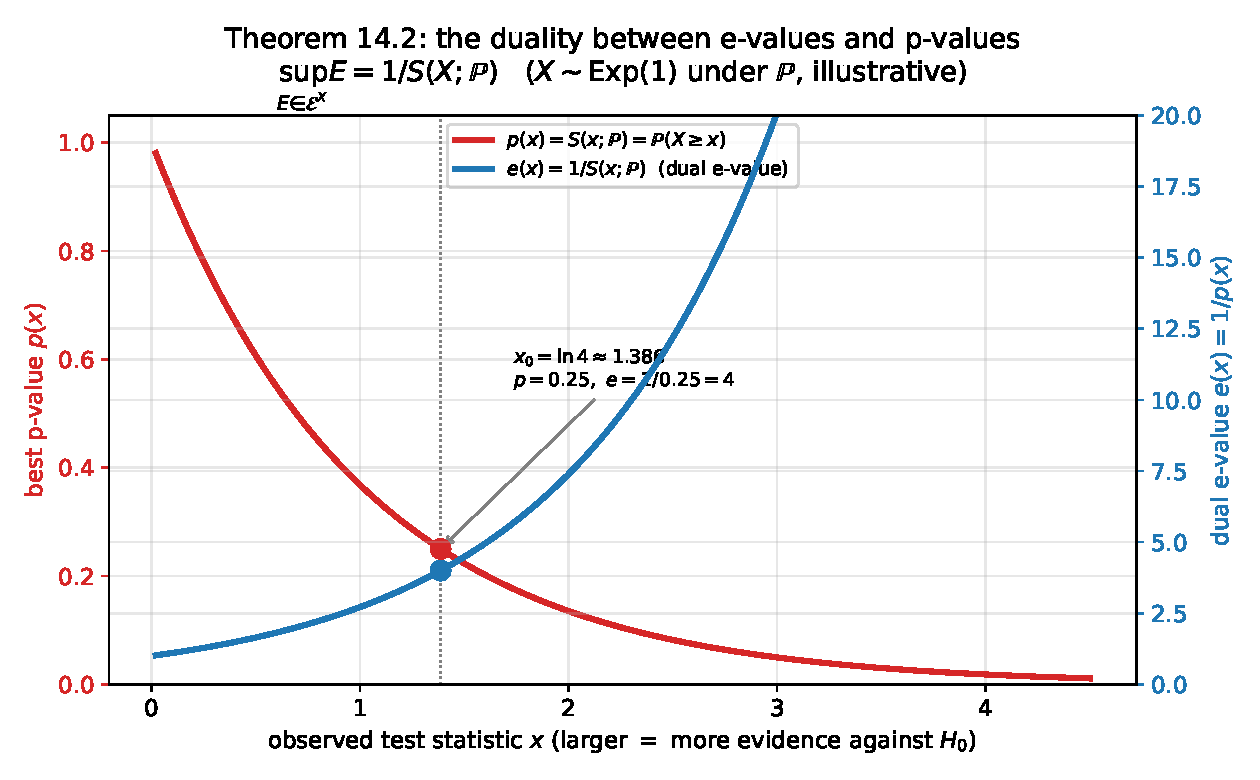
\includegraphics[width=0.82\textwidth]{fig1_duality_curve.pdf}

  \small As the test statistic $x$ grows, the best p-value $S(x;\PP)$
  decreases while the dual e-value $1/S(x;\PP)$ increases -- they are
  reciprocal curves, matching at $p=0.25 \leftrightarrow e=4$.
\end{frame}

\begin{frame}[fragile]{Python: the duality map numerically}
  \begin{lstlisting}
import numpy as np

rng = np.random.default_rng(0)

def S(x):                       # survival fn of X ~ Exp(1) under P
    return np.exp(-x)

# --- duality map e(x) = 1 / S(x;P), for several observed x ---
for x in [0.5, 1.0, 1.386, 2.0, 3.0]:
    p = S(x)            # best (smallest) p-value at this x
    e = 1.0 / p          # dual (largest) e-value, Theorem 14.2
    print(f"x={x:5.3f}  p=S(x)={p:.4f}  e=1/p={e:8.3f}")

# --- concrete check: e = 4  <->  p = 0.25 ---
x0 = -np.log(0.25)               # solve exp(-x0) = 0.25
print("x0 with p=0.25:", round(x0, 4), " -> e =", 1 / 0.25)

# --- Monte Carlo check of Corollary 14.3 (Ville/Markov bound) ---
N = 200_000
X = rng.exponential(scale=1.0, size=N)
alpha = 0.1
E = 1.0 / S(X)                     # the extremal e-variable sup_s E_s
empirical = np.mean(E >= 1 / alpha)
print("P(E >= 1/alpha) empirical:", round(empirical, 4),
      " <= alpha =", alpha)
  \end{lstlisting}
  \small Output confirms $e(x_0{=}1.386)\approx 4.00$ and the empirical
  tail probability sits at (or just below) $\alpha = 0.1$, consistent with
  Corollary 14.3.
\end{frame}

\begin{frame}[allowframebreaks]{Corollary 14.3: a strengthened Ville/Markov bound}
  \textbf{Intuition.} Ordinary Markov's inequality for a single e-variable
  $E$ says $\PP(E \geq 1/\alpha) \leq \alpha$. Because the duality theorem
  produces an explicit \emph{extremal} e-variable dominating an entire
  family $\calE$ at once, we get a uniform version: the supremum over a
  whole comonotonic family of e-variables still only breaches $1/\alpha$
  with probability at most $\alpha$.

  \begin{block}{Corollary 14.3}
    For any set $\calE$ of e-variables for $\calP$ that are increasing
    functions of $X$,
    \[
      \sup_{\PP\in\calP} \PP\left(\sup_{E\in\calE} E \geq \frac{1}{\alpha}\right) \leq \alpha
      \qquad \text{for all } \alpha \in (0,1).
    \]
    \emph{Symbols:} $\calE$ = any collection of monotone e-variables (not
    just one); the bound holds for the \emph{supremum} of the whole
    collection simultaneously, uniformly over $\PP \in \calP$.
  \end{block}

  \framebreak

  \textbf{Why this is stronger than plain Markov.} Applying Markov's
  inequality to each $E \in \calE$ separately and union-bounding over
  $|\calE|$ elements would cost a factor of $|\calE|$ (or require a
  Bonferroni correction). Corollary 14.3 needs no such correction: because
  every $E \in \calE^X$ is dominated $\PP$-a.s.\ by the single random
  variable $1/S(X;\PP)$ (Theorem 14.2), the event
  $\{\sup_{E} E \geq 1/\alpha\}$ is itself controlled by the tail of
  $S(X;\PP)$, and no union bound is needed.

  \textbf{The key structural reason: comonotonicity.} What actually
  matters for this ``free lunch'' is that all e-variables under
  consideration are \emph{comonotonic} -- increasing functions of the
  \emph{same} random variable $X$ (or all decreasing in $X$; monotonicity
  can be flipped throughout by using the right-continuous survival
  function instead). Chapter 15.2 develops this comonotonicity idea more
  generally.
\end{frame}

% ============================================================
\section{14.2 Representations as conditional expectations/probabilities}
% ============================================================

\begin{frame}{14.2 Motivation: what is an e-value, structurally?}
  \textbf{Intuition.} So far, e-variables have been defined by an
  \emph{inequality}: $\EE^{\PP}[E] \leq 1$. This section shows something
  stronger and more structural: every e-variable is (dominated by) an
  actual \textbf{conditional expectation} of a likelihood ratio
  $d\QQ/d\PP$ given the data. Likewise, every p-variable is (dominated by)
  an actual \textbf{conditional probability}. This is a deeper fact than
  the defining inequalities alone -- it explains why the letter ``e''
  stands for \emph{expectation}.

  \textbf{Setup.} Let $X$ be a generic data sample (a measurable map into
  $\RR^n$; the ambient space plays no role here). A p- or e-variable $Y$
  is \emph{built on $X$} if it is a measurable function of $X$ -- i.e.\
  $Y$ only depends on the data through $X$.
\end{frame}

\begin{frame}[allowframebreaks]{Theorem 14.4: e-variables are conditional expectations}
  \begin{block}{Theorem 14.4 (Representation for e-variables)}
    For a random variable $E$, the following are equivalent:
    \begin{enumerate}
      \item[(i)] $E$ is an e-variable for $\calP$ built on $X$;
      \item[(ii)] for every $\PP \in \calP$, there exists a probability
        measure $\QQ \ll \PP$ such that
        \[
          E \ \leq\ \EE^{\PP}\!\left[\frac{d\QQ}{d\PP} \,\Big|\, X\right]
          \qquad \PP\text{-almost surely.} \tag{14.2}
        \]
    \end{enumerate}
    If all $\PP \in \calP$ are equivalent to some measure $\mathbb{L}$,
    every e-variable built on $X$ is dominated by
    \[
      \inf_{\PP\in\calP} \EE^{\PP}\!\left[\frac{d\QQ_{\PP}}{d\PP}\,\Big|\,X\right],
    \]
    itself an e-variable for $\calP$, for some class $(\QQ_{\PP})_{\PP\in\calP}$
    absolutely continuous w.r.t.\ $\mathbb{L}$.
    \emph{Symbols:} $d\QQ/d\PP$ is the Radon--Nikodym derivative
    (likelihood ratio) of an \emph{alternative} $\QQ$ against the null
    $\PP$; conditioning on $X$ averages this ratio over whatever
    additional randomness is not captured by $X$.
  \end{block}

  \framebreak

  \textbf{A familiar special case.} When densities exist (Chapter 5), the
  conditional expectation in (14.2) often reduces to
  \[
    \EE^{\PP}\!\left[\frac{d\QQ}{d\PP}\,\Big|\,X\right] = \frac{p(X)}{q(X)},
  \]
  where $p, q$ are the densities of $X$ under $\PP, \QQ$: exactly the
  ordinary \emph{likelihood ratio} test statistic.

  \textbf{Step-by-step derivation.}
  \begin{enumerate}
    \item \emph{(ii)$\Rightarrow$(i).} By the tower property of
      conditional expectation, for every $\PP \in \calP$,
      \[
        \EE^{\PP}[E] \leq \EE^{\PP}\!\left[\EE^{\PP}\!\left[\frac{d\QQ}{d\PP}\,\Big|\,X\right]\right]
        = \EE^{\PP}\!\left[\frac{d\QQ}{d\PP}\right] = 1.
      \]
      So $E$ satisfies the e-variable inequality for every $\PP$.
    \item \emph{(i)$\Rightarrow$(ii).} Fix $\PP\in\calP$. If
      $\EE^{\PP}[E] > 0$, define $\QQ$ by
      \[
        \frac{d\QQ}{d\PP} = \frac{E}{\EE^{\PP}[E]};
      \]
      this is a valid density since it is $\geq 0$ with $\PP$-expectation
      $1$. If $\EE^{\PP}[E] = 0$, just set $\QQ = \PP$.
    \item \emph{Verify (14.2) holds with equality-or-more.} For $\PP$ with
      $\EE^{\PP}[E] > 0$,
      \[
        \EE^{\PP}\!\left[\frac{d\QQ}{d\PP}\,\Big|\,X\right]
        = \EE^{\PP}\!\left[\frac{E}{\EE^{\PP}[E]}\,\Big|\,X\right]
        = \frac{E}{\EE^{\PP}[E]} \geq E \qquad (\text{since } \EE^{\PP}[E]\leq 1).
      \]
      For $\PP$ with $\EE^{\PP}[E]=0$, $E=0$ $\PP$-a.s., and (14.2) holds
      trivially since the right side is $\geq 0 = E$.
  \end{enumerate}

  \textbf{Takeaway.} Every e-value \emph{is}, structurally, a (bounded
  version of a) conditional expectation of some likelihood ratio -- not
  merely a number satisfying an expectation constraint. Theorem 14.4
  generalizes the simple-null likelihood-ratio connection from
  Proposition 2.12 to arbitrary composite $\calP$.
\end{frame}

\begin{frame}[allowframebreaks]{Theorem 14.5: p-variables are conditional probabilities}
  \textbf{Intuition.} The mirror-image fact holds for p-values: a
  p-variable is (dominated by) the conditional probability that an
  independent replicate of the data looks ``at least as extreme'' as what
  was observed -- precisely capturing the everyday informal description
  of a p-value.

  \begin{block}{Theorem 14.5 (Representation for p-variables)}
    For a random variable $P$, the following are equivalent:
    \begin{enumerate}
      \item[(i)] $P$ is a p-variable for $\calP$ built on $X$;
      \item[(ii)] there exists a measurable $T:\RR^n\to\RR$ such that, for
        every $\PP\in\calP$,
        \[
          P \ \geq\ \PP\big(T(X') \leq T(X) \mid X\big) \qquad \PP\text{-a.s.}, \tag{14.3}
        \]
        where $X'$ is an i.i.d.\ copy of $X$ under $\PP$.
    \end{enumerate}
    If all $\PP\in\calP$ are equivalent to some $\mathbb{L}$, every
    p-variable built on $X$ is dominated by (i.e.\ $\leq$)
    \[
      \sup_{\PP\in\calP} \PP\big(T(X'_{\PP}) \leq T(X) \mid X\big),
    \]
    itself a p-variable for $\calP$.
    \emph{Symbols:} $T$ = a test statistic (possibly different from $X$
    itself); $X'$ = a fresh independent draw under the \emph{same} $\PP$
    used for conditioning.
  \end{block}

  \framebreak

  \textbf{Step-by-step derivation.}
  \begin{enumerate}
    \item \emph{(ii)$\Rightarrow$(i).} Fix $\PP$, let $F_T$ be the cdf of
      $T(X)$ under $\PP$. Since $X'\sim X$ under $\PP$,
      \[
        \PP(T(X')\leq T(X)\mid X) = F_T(T(X)).
      \]
      A standard probability fact: for any real random variable $Z$ with
      cdf $F$, $\PP(F(Z) \leq \alpha) \leq \alpha$. Applying this with
      $Z=T(X)$, $F=F_T$ gives $\PP(P\leq\alpha)\leq \PP(F_T(T(X))\leq\alpha)\leq\alpha$,
      so $P$ is a p-variable.
    \item \emph{(i)$\Rightarrow$(ii).} Take $T(X) := P$ (treat $P$ itself
      as the statistic). Let $F_P$ be $P$'s cdf under $\PP$. Since $P$ is
      a p-variable, by definition $F_P \leq \mathrm{id}$ on $[0,1]$, so
      \[
        P \ \geq\ F_P(P) \ =\ \PP(T(X')\leq T(X) \mid X).
      \]
  \end{enumerate}

  \textbf{Takeaway.} A p-value \emph{is}, structurally, the (bound on the)
  conditional probability that a fresh replicate's test statistic is no
  more extreme than the one observed -- exactly the textbook interpretation
  of a p-value, now made rigorous for arbitrary composite nulls.
\end{frame}

\begin{frame}{Side-by-side: e-value vs.\ p-value, structurally}
  \centering
  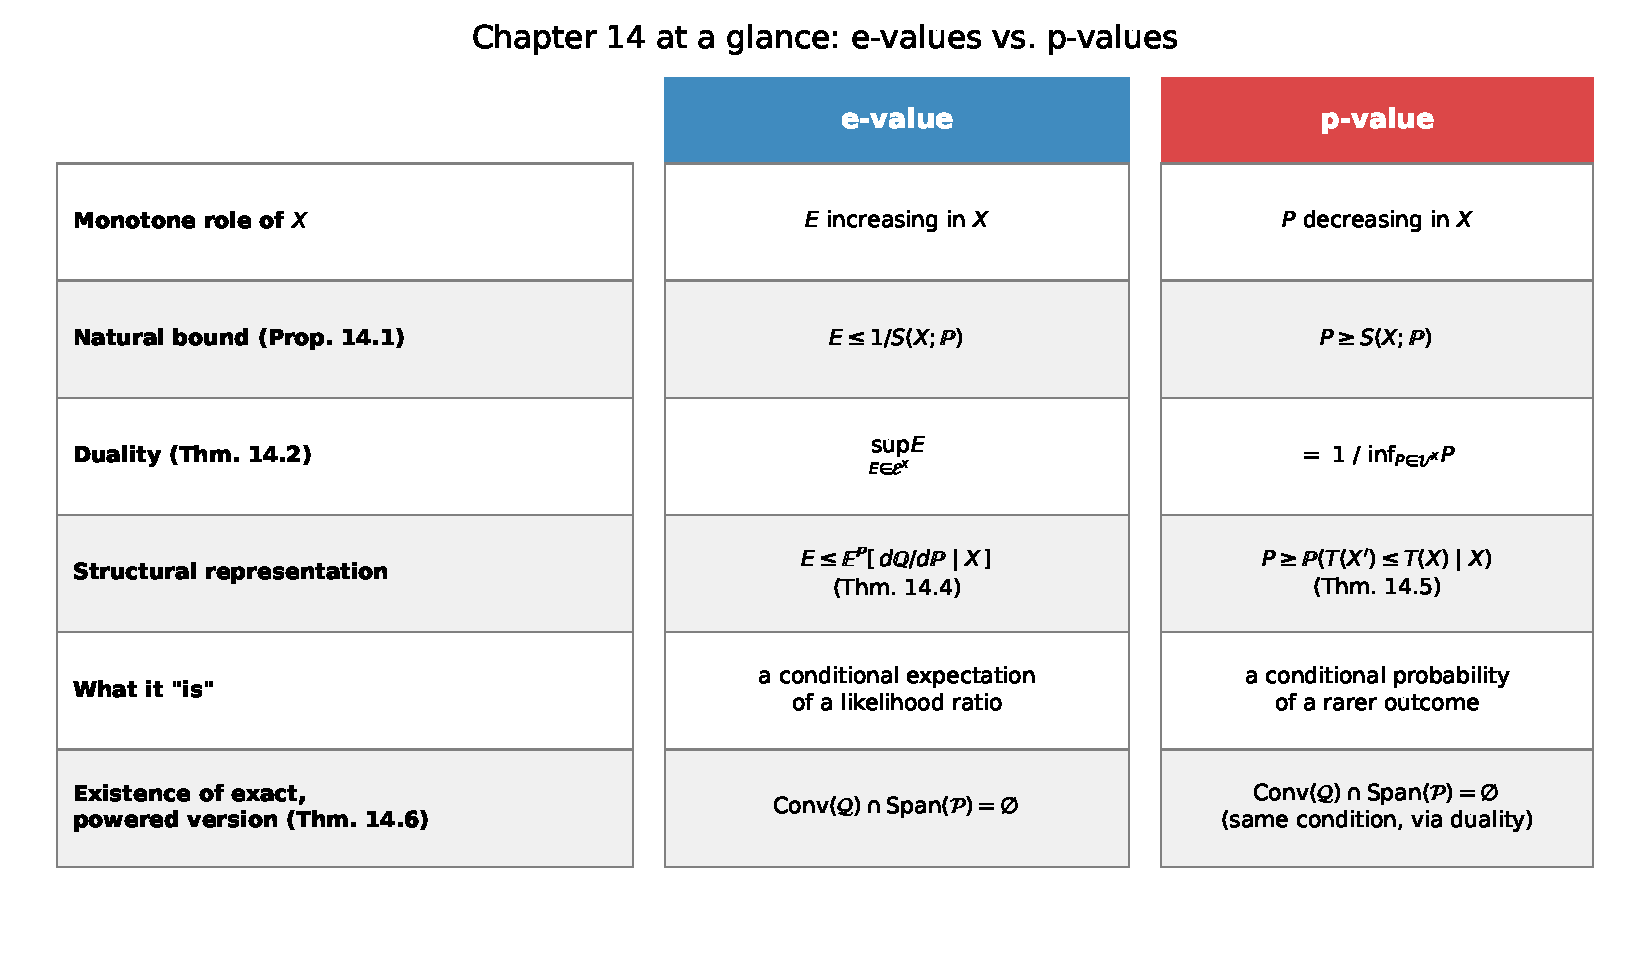
\includegraphics[width=0.92\textwidth]{fig2_contrast_panel.pdf}

  \small e-values are conditional \emph{expectations} of likelihood
  ratios; p-values are conditional \emph{probabilities} of exceedance
  events. The duality of Section 14.1 and the existence result of
  Section 14.3 sit on top of this same expectation/probability contrast.
\end{frame}

% ============================================================
\section{14.3 Existence of powered exact e-values and p-values}
% ============================================================

\begin{frame}{14.3 Setup: finite hypotheses, pivotal statistics}
  \textbf{Intuition.} Chapter 3 asked: when does a powered (nontrivial)
  e-value exist at all against a given alternative? Section 14.3 asks the
  sharper question: when does an \emph{exact} e-value (or, equivalently,
  an exact p-value) that is also powered exist, when both null and
  alternative are finite collections of distributions?

  \begin{block}{Definitions}
    For a finite null $\calP=\{\PP_1,\dots,\PP_L\}$, a random variable $X$
    is \textbf{pivotal} if it has the \emph{same} distribution under every
    $\PP \in \calP$. Recall an e-variable is \textbf{exact} if
    $\EE^{\PP}[E]=1$ for every $\PP\in\calP$ (then $E$ is automatically
    pivotal-compatible), and a p-variable is \textbf{exact} if it is
    exactly $\mathrm{Uniform}[0,1]$ under every $\PP\in\calP$.
  \end{block}

  Being \emph{powered against} a finite alternative
  $\calQ=\{\QQ_1,\dots,\QQ_M\}$ means the e-value has expectation $>1$
  (resp.\ the p-value rejects with nontrivial probability) under every
  $\QQ \in \calQ$.
\end{frame}

\begin{frame}[allowframebreaks]{Theorem 14.6: the existence condition}
  \begin{block}{Theorem 14.6}
    Consider testing a finite $\calP=\{\PP_1,\dots,\PP_L\}$ against a
    finite $\calQ=\{\QQ_1,\dots,\QQ_M\}$. Under a regularity condition
    (U) permitting external randomization, the following are equivalent:
    \begin{enumerate}
      \item[(i)] there exists an exact (hence pivotal) p-variable that is
        powered against $\calQ$;
      \item[(ii)] there exists a pivotal, exact, bounded e-variable with
        positive e-power against $\calQ$;
      \item[(iii)] there exists an exact e-variable that is powered
        against $\calQ$;
      \item[(iv)] $\Conv(\QQ_1,\dots,\QQ_M) \cap \Span(\PP_1,\dots,\PP_L) = \varnothing$.
    \end{enumerate}
  \end{block}

  \begin{block}{Span vs.\ convex hull}
    \[
      \Span(\PP_1,\dots,\PP_L) = \left\{ \sum_{\ell=1}^L \lambda_\ell \PP_\ell \ :\ \lambda_\ell \in \RR \text{ for each } \ell \right\},
    \]
    a set of \emph{signed} measures, allowing \emph{any real} coefficients
    $\lambda_\ell$ (not requiring $\lambda_\ell\geq 0$ or $\sum_\ell\lambda_\ell=1$
    as the convex hull would). \emph{Symbols:} $\Conv(\QQ_1,\dots,\QQ_M)$
    is the usual convex hull (probabilistic mixtures) of the alternative;
    the null side is enlarged all the way to its linear span.
  \end{block}

  \framebreak

  \textbf{Why the span appears: step-by-step intuition for (iii)$\Rightarrow$(iv).}
  \begin{enumerate}
    \item Suppose an exact e-variable $E$ is powered against $\calQ$, so
      $\EE^{\QQ}[E] > 1$ for every $\QQ$ in the convex hull
      $\Conv(\calQ)$ (expectation is linear, so powered against the
      extreme points $\QQ_1,\dots,\QQ_M$ implies powered against all
      mixtures).
    \item Suppose, for contradiction, some $\QQ_0 \in \Conv(\calQ)$ can
      also be written as a \emph{signed} linear combination of the null
      measures,
      \[
        \QQ_0 = \sum_{\ell=1}^L \lambda_\ell \PP_\ell, \qquad \lambda_\ell \in \RR.
      \]
      Because $\QQ_0$ is a probability measure and each $\PP_\ell$
      integrates to 1, applying both sides to the whole sample space
      forces $\sum_{\ell=1}^L \lambda_\ell = 1$.
    \item Then, using linearity of expectation and \emph{exactness} of
      $E$ (i.e.\ $\EE^{\PP_\ell}[E] = 1$ for every $\ell$),
      \[
        \EE^{\QQ_0}[E] = \sum_{\ell=1}^L \lambda_\ell\, \EE^{\PP_\ell}[E]
        = \sum_{\ell=1}^L \lambda_\ell \cdot 1 = \sum_{\ell=1}^L \lambda_\ell = 1.
      \]
    \item This contradicts $\EE^{\QQ_0}[E] > 1$ from step 1. Hence no
      such signed representation $\QQ_0 = \sum_\ell \lambda_\ell \PP_\ell$
      can exist, i.e.\
      $\Conv(\calQ) \cap \Span(\PP_1,\dots,\PP_L) = \varnothing$.
  \end{enumerate}

  \framebreak

  \textbf{Comparison with Theorem 3.9.} The basic existence result for
  (inexact) powered e-values in Chapter 3 required
  $\Conv(\QQ_1,\dots,\QQ_M) \cap \Conv(\PP_1,\dots,\PP_L) = \varnothing$
  -- disjointness from the \emph{convex hull} of the null. Theorem 14.6
  replaces $\Conv(\calP)$ by the strictly larger $\Span(\calP)$ (allowing
  negative and unnormalized coefficients), which is a \emph{harder}
  condition to satisfy -- reflecting the fact that requiring
  \emph{exactness} (not just $\EE^{\PP}[E]\le 1$) is a real restriction.

  A full proof of Theorem 14.6 needs tools from optimal transport theory
  and is not reproduced here; only the intuitive direction
  (iii)$\Rightarrow$(iv) is elementary, as shown above.
\end{frame}

\begin{frame}{Chapter 14 takeaways}
  \begin{itemize}
    \item \textbf{Duality (14.1).} For monotone transforms of one test
      statistic $X$, the best e-value and best p-value are exact
      reciprocals: $\sup_{E\in\calE^X} E = 1/\inf_{P\in\calU^X} P$
      $\mathbb{L}$-a.s.\ (Theorem 14.2), sharpening Markov's inequality to
      a uniform, union-bound-free statement (Corollary 14.3).
    \item \textbf{Structural representations (14.2).} Every e-variable is
      dominated by a conditional expectation $\EE^{\PP}[d\QQ/d\PP\mid X]$
      of a likelihood ratio (Theorem 14.4); every p-variable is dominated
      by a conditional probability $\PP(T(X')\leq T(X)\mid X)$ of a
      replicate being no more extreme (Theorem 14.5).
    \item \textbf{Existence with exactness (14.3).} For finite hypotheses,
      an exact, powered e-value (equivalently p-value) exists iff
      $\Conv(\calQ) \cap \Span(\calP) = \varnothing$ (Theorem 14.6) --
      the span, not the convex hull, of the null is the right geometric
      object once exactness is demanded.
  \end{itemize}
\end{frame}

\end{document}
